
\chapter{词法,语法与语义分析}
\label{basic} % Always give a unique label
% use \chaptermark{}
% to alter or adjust the chapter heading in the running head

\section{词法分析}
\subsection{问题定义}
词法分析是自然语言处理的第一步,要做NLP深层次分析,比如句法分析、语义分析,甚至NLP复杂应用的先决条件,就是首先进行词法分析。词法分析的核心是,将自然语言解析为一个个词的序列,并判断每个词的词性、专名信息,为后续分析做好准备。总的来说,在中文这种孤立语中,词法分析主要由分词、词性标注、命名实体识别3个子任务组成。在英语、阿拉伯语等屈折语中,词法分析一般还包括词根还原(word stemming)任务。忽略词根还原,词法分析可以归纳为3个具体的子任务:

\begin{itemize}
\item 自动分词(word segmentation):是将连续的自然语言文本,切分成具有语义合理性和完整性的词汇序列的过程。
\item 词性标注(Part-of-Speech tagging):是指为自然语言文本中的每个词汇赋予一个词性的过程。
\item 命名实体识别(Named Entity Recognition,也称专名识别):是指识别自然语言文本中具有特定意义的实体,主要包括人名、地名、机构名、时间日期等。
\end{itemize}

\begin{figure}[h!]
\centering
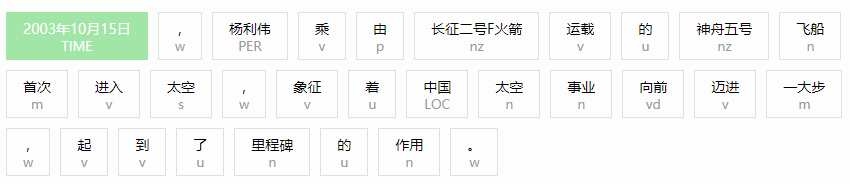
\includegraphics[scale=0.5]{img/chapter_nlp/lexical_example.png}
\caption{词法分析示例}
\label{fig:lexical_example}
\end{figure}

如图\ref{fig:lexical_example}所示,将输入句子切分成一个个词汇,然后给每个词汇标记出名词、动词、介词等词性;并且识别出“2003年10月15日”是一个时间专名,识别“杨利伟”是一个人名专名等。

因为词法分析的自动分词、词性标注、专名识别本质上是类似的,所以它们的发展历史方也是类似的。总结起来,都大致经历词典匹配、机器学习、深度学习这3个发展阶段。

\subsection{实现方案}

\subsubsection{词典匹配}
\noindent
基于词典匹配的实现步骤:

\begin{enumerate}
\item 词典构建:根据具体子任务的语言学知识构建词典。如果是自动分词,则收录常见的词条短语;如果是词性标注、专名识别,则收录当前常见词条对应的名词、动词、介词、专名类型等属性,并且保留相应词性、专名属性的概率。词典构建,通常需要人工收集、整理、离线更新,维护成本较高。
\item 词典匹配:扫描输入的所有子序列,如果当前子序列能够匹配词典中某个词条,则当前子序列属一个可能的候选。如果是分词,则当前子序列就可能为一个分词的词汇;如果是词性标注、专名识别,则当前子序列以相应的概率取词典中的词条属性。
\item 歧义消解:由于候选子序列之间存在歧义,所以基于词典匹配之上,需要加入一些启发式规则以解决歧义问题。常用规则主要包含最大前向匹配(Forward Maximum Matching,FMM)、最大后向匹配(Backward Maximum Matching,BMM)、最少切分、双向最大匹配、长片段优先等策略\cite{wong1996chinese}\cite{weichun2013research}。
\end{enumerate}

中文分词如图\ref{fig:word_segmentation_example}所示。输入序列进行词典匹配之后,得到对应的DAG图,图中每条边都是词典词条,边的权重都为1,图中每一种首尾贯通的连接都是一种歧义切分的候选结果。比如由此只要求解DAG图的最优路径,则可以得到输入序列对应的分词结果。

\begin{figure}[h!]
\centering
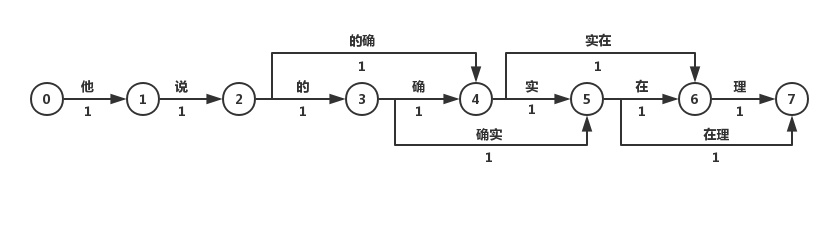
\includegraphics[scale=0.4]{img/chapter_nlp/word_segmentation_example.jpg}
\caption{中文分词示例}
\label{fig:word_segmentation_example}
\end{figure}

很长一段时间内研究者都在对基于词典匹配方法进行优化,比如最大长度设定、字符串存储和查找方式以及对于词表的组织结构,比如采用TRIE索引树\cite{yang2012enhanced}、哈希索引\cite{li2003new}等、AC自动机\cite{ngword}等结构方便快速查找。

基于词典匹配的优缺点:
\begin{itemize}
\item 优点:实现简单、运行速度快
\item 缺点:面临词典收录更新困难、未登录词难处理;同时由于消除歧义策略过于简单,通常效果不甚理想。
\end{itemize}

\subsubsection{机器学习}
\noindent
基于机器学习的实现步骤:

\begin{enumerate}
\item 转换为序列标注任务:词法分析3个子任务,都通过定义标注空间标签集,将具体任务转换为标准序列标注任务。以中文分词为例:转换方法为,标注每个字在其所属词中的位置。因为对于任何一个字来说,它可以是一个词的开始(Begin), 一个词的中间(Inside), 一个词的结尾(End),或者本身就是一个单字的词(Singleton),这也就是在分词序列标注中常用的BIES的分类。只需将输入序列的每个字标上BIES标签中的一个,就可以转换得到对应的分词结果。这种标注空间(模型状态空间)的划分在词性标注和专名识别任务上也很常用,也会有一些类似的变种,比如专名识别中常用BIO标签集。
\item 求解序列标注任务:传统序列标注模型主要包括隐马尔科夫模型(Hidden Markov Model)\cite{zhang2003chinese}\cite{kupiec1992robust}\cite{yu2006chinese}\cite{morwal2012named}、最大熵马尔科夫模型(Maximum Entropy Markov Model)\cite{mccallum2000maximum}\cite{ratnaparkhi1996maximum}\cite{borthwick1999maximum}、条件随机场(Conditional Random Field)\cite{zhao2006improved}\cite{constant2011mwu}\cite{ekbal2008named}、结构化感知机(Structural Perception Machine)\cite{zhang2007chinese}\cite{zhang2008joint}等浅层模型。这些浅层模型的区别主要在于如何对待输入字序列和标签序列之间的概率,训练目标是最大联合概率似然、最大条件概率似然,还是最小化风险等。
\end{enumerate}

总结来说:传统序列标注模型中,CRF是集大成者。相比于HMM,CRF去除了输出独立性要求,对于整个序列内部的信息和外部观测信息都可以有效利用,可以更加有效建模上下文。相比于MEMM,CRF通过全局归一化(global normalization),避免了MEMM locally normalized导致的label bias缺陷。

以自动分词任务为例,则其序列标注任务定义为:
定义标签集为$L=\{B, I, E, S\}$,给定输入文本序列$X=\{x_{1}, x_{2}, ..., x_{n}\}$,目标是求解最优标注序列$Y^{*}=\{y^{*}_{1}, y^{*}_{2}, ..., y^{*}_{n}\}$:

\[y^{*}=\mathop{\arg\max}\limits_{Y \in L^{n}} p(\bm{Y}|\bm{X})\]

预测时,使用维特比算法求解最优标注序列$Y^{*}$;训练时,使用最大化条件似然来训练模型,其中,$f_{i}$为人工定义的特征函数:

\[P_{w}(Y|X)=\frac{1}{Z_{w}(x)}\exp(\sum_{i} w_{i} f_{i}(y_{i}, y_{i-1}, x))\]

\[Z_{w}(x)=\sum\limits_{y \in Y}\exp(\sum_{i} w_{i} f_{i}(y_{i}, y_{i-1}, x))\]

\noindent
基于机器学习的优缺点:
\begin{itemize}
\item 优点:通过人工设计的特征工程,充分地挖掘了序列的上下文信息。模型的歧义消解胜过词典匹配的方法;同时具有很强的泛化能力,能够很好地处理未登录词问题。
\item 缺点:特征工程不经需要耗费大量人力,而且需要大量语言学知识,设计和寻找有效特征存在较高门槛;另外,这些浅层模型,通常使用离散的binary特征,无法表达复杂先验,比如没法利用词向量。
\end{itemize}

\subsubsection{深度学习}
随着大数据、神经网络、深度学习的快速发展,很多研究提出利用前馈神经网络来解决词法分析\cite{collobert2011natural}\cite{zheng2013deep}任务。总的来说,与前面基于机器学习的方法类似,也是把词法分析任务作为序列标注问题进行求解,只是把人工设计特征函数,改成了使用多层前馈神经网络进行自动特征抽取。

\begin{figure}[h!]
\centering
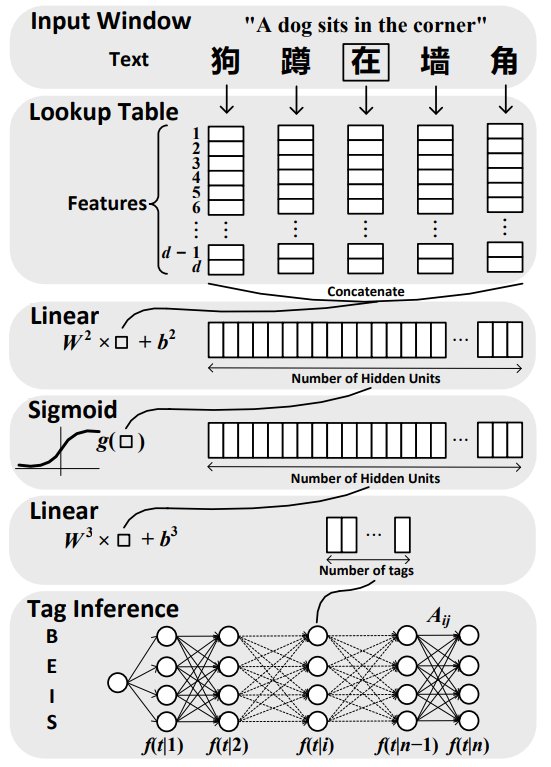
\includegraphics[scale=0.5]{img/chapter_nlp/dl_segmentation_example.png}
\caption{深度学习分词示例}
\label{fig:dl_segmentation_example}
\end{figure}

如图\ref{fig:dl_segmentation_example}所示,网络的第一层输入句子中每个字的字向量,第二层将一个固定长度的字向量进行拼接,然后输入到标准前馈神经网络结构中,神经网络输出在标注集合上的lattice,最后利用维特比算法进行解码,就可以得到最优标注序列。

后续有很多研究,深度学习框架基础上,对前馈神经网络进行改进,进一步探索了卷积神经网络\cite{wu2019neural}、循环神经网络\cite{chen2015long}、递归神经网络\cite{chen2015gated}等复杂结构对词法分析任务的影响。

另外,传统的词法分析通常会把分词、词性标注、命名实体识别当成pipeline形式的进行处理,这样带来的一个问题就是错误传播。比如,分词的错误将会导致后续词性标注、专名识别、句法分析、语义分析出现错误。所以在学术界也有很多联合建模\cite{zhang2008joint}\cite{hatori2012incremental}\cite{shao2017character}方面的工作。联合建模的一大好处是词法分析与其他任务可以共享有用的信息,词法分析的时候也会考虑到其他任务的要求,其他任务也会考虑各种词法分析的可能性,通常可以再全局上取得最优解。但是随之而来问题是搜索的复杂度往往会显著提高:需要更有效的搜索剪枝机制在控制复杂度的同时,不对搜索的结果产生显著影响。

值得一提的是,2018年Peters等证明在预训练语言模型\cite{conneau2017supervised}\cite{mccann2017learned}\cite{subramanian2018learning},在各种NLP任务中提供比最先进的技术更大的改进。可以将语言模型嵌入作为特征,使用目标任务数对语言模型对进行微调\cite{ramachandran2016unsupervised}\cite{howard2018universal},通常就能达到或超过传统结果。由于语言模型只需要无标记的数据便可以进行学习,因此对于标记数据稀缺的低资源场景,预训练语言模型尤其有用。

总结起来,基于深度学习方法的优点是通过深度神经网络自动学习多层特征抽象,避免了复杂的特征工程;模型的歧义消解、泛化能力通常都很好。只是,深度学习模型需要训练充分,通常对数据量、计算量都有较高的要求。

\subsection{应用案例}
通常NLP中深层次的语法语义分析通常都是以词作为基本单位,所以词法分析都是这些深层次分析的基础和先决条件。词法分析作为自然语言处理的第一步,是下游所有分析任务的基础。这些下游应用小句法分析、语义分析,大到对话系统、文本分类、自动摘要、机器翻译\cite{chang2008optimizing}、信息检索、搜索引擎、语音合成等等。几乎只要有利用到自然语言处理技术的地方,词法分析都是不可或缺的基础技术。

比如在搜索引擎中,用户输入一个表述需求信息的查询字段,系统回复一个包含所需要信息的文档列表。其核心技术在于索引构建和相关性计算。

索引构建:首先需要对互联网海量文档进行,分词、词性标注、专名识别;利用词法分析的结果,以词为粒度,为所有文档建立倒排索引。

相关性计算:首先需要对用于查询字段进行词法分析,找出表达用户需求的核心词汇;然后以这些核心词汇为key,去拉取相应的倒排索引,获取初步筛选后的文档;接着,为了要提高返回结果的相关性,需要计算用户查询和初筛文档之间的相似度,取相似度较好的文档返回。其中计算用户查询和文档之间的相似度,通常利用BM25、语义计算等技术,而它们也都是以词为单位进行的,由此看出词法分析在搜索引擎中的重要性、基础性。

在比如在文本分类和情感分类中,在预定义分类体系下,输入给定文本,抽取文本特征,将给定文本于一个或多个类别相关联的过程。其中,抽取文本特征的时候,通常也都是先进行词法分析,先获得给定文本的词汇、词性、专名等信息,然后以词汇为单位,以词汇的词向量、词性专名等信息为特征,利用机器学习、深度学习的分类模型进行预测。


\section{语法分析}
\subsection{问题定义}
短语结构语法(Constituency Structure Grammar)和依存关系语法(Dependency Grammar)是现在常见的两种语法关系。短语结构语法又叫上下文无关文法 (Context-Free Grammars,CFGs),它从一个特殊的初始符号出发,不断的应用一些产生式规则,从而生成出一个字串的集合(如句子)。产生式规则指定了某些符号组合如何被另外一些符号组合替换。
它呈现一个树分类关系,句法根据一定的规则进行转换分析。每一个词的转换都是需要按照设定的树值规则进行目的性的转换。

依存语法(从属关系语法) 是由法国的语言家Lucien Tesnière提出的\cite{tesniere1959elements},
它将句子各个词语之前的搭配关系描述成预先定义好的依存关系。它基于一个基本假设:句法结构本质上包含词和词之间的依存(修饰)关系。一个依存关系连接两个词,分别是核心词(head)和依存词(dependent)。依存关系可以细分为不同的类型,表示两个词之间的具体句法关系。比如主语依赖于谓语(SBV),宾语也依赖于谓语(VOB)以及定语依赖于名词性短语(ATT)等。依存句法认为“谓语”中的动词是一个句子的中心,其他成分与动词直接或间接地产生联系。

除了以上介绍的两种句法体系外,国内外都开展了对句法分析的研究。不论是国外的链语法(Link Grammar) 、组合范畴语法(Combinatory categorial grammar,CCG)等,还是国内黄曾阳教授提出的HNC理论(Hierarchical Network of Concept)\cite{黄曾阳:12}都是目前行业内常用的语法,只是由于设定区域的不同,所以使用有一定的局限性。

短语结构分析的语法集是由固定的语法集组成,较为固定和呆板,依存语法则更加的自由。另外依存语法树标注简单且parser准确率更高,再加之通用依存数据集(Universal Dependencies Treebanks)的发展,依存语法分析受到专家学者普遍的青睐,得到越来越多的应用。这里也将着重介绍依存语法分析。

\begin{figure}[h]
\centering
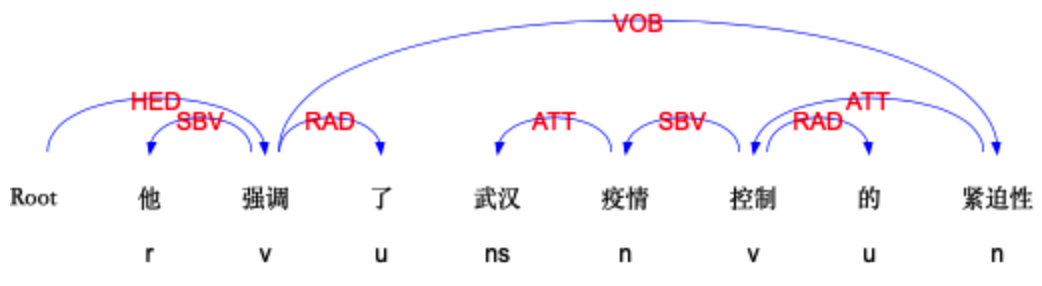
\includegraphics[scale=0.3]{img/chapter_nlp/parser_example.png}
\caption{LTP依存句法分析样例}
\label{fig:parserexample}
\end{figure}
例如,从上述例子中我们可以看到,句子的核心谓词为“强调”,主语(SBV)是“他”,强调的宾语(VOB)是“紧迫性”,“紧迫性”的修饰语(ATT)是“武汉疫情控制”。


\subsection{实现方案}
依存句法分析方法主要可以分为两种,一种是基于图的方法(Graph Based),一种是基于转移(Transition Based)的方法。基于图的方法先建立句子中所有词语的全连接图,然后求图中的最大生成树。 两种方法中更主流的算法是基于转换的依存句法分析,基于转移的方法将依存树的构成过程建模为一个动作序列,将依存分析问题转化为寻找最优动作序列的问题。通过 SHIFT, LEFT\_ARC, RIGHT\_ARC三个动作来将序列转换为树结构。一次分析任务$C = (s, b, A)$由一个Stack栈 $s$,一个buffer缓冲区 $b$,一系列依存弧列表$A$构成。初始化栈$s$里面只包含一个$root$元素即根元素,$s_1$代表栈顶元素,$s_2$表示栈顶第二个元素。缓冲区$b$是一个队列,里面包含了要解析的一句话的序列,$A$为空。一条依存弧有两个信息:动作类型+依存关系名称$l$。$l$视依存句法语料库中使用了哪些依存关系label而定。动作SHIFT将缓冲区$b$ 中最上面的一个词$b_1$移到stack中,即不建立依存关系,只转移句法分析的焦点,即新的左焦点词是原来的右焦点词,依此类推。LEFT\_ARC,即添加栈顶两个词 $s_1$,$s_2$之间的依存边,方向为$s_1 \rightarrow s_2$,并且将$s_2$ 从栈$s$中删除。RIGHT\_ARC,即添加栈顶两个词 $s_1$,$s_2$之间的依存边,方向为$s_2 \rightarrow s_1$,并且将$s_1$ 从栈$s$中删除。

比如图\ref{fig:parserexample}中,首先模型判断执行SHIFT动作将“他”移到栈$s$上,然后再执行SHIFT动作将“强调”移到 栈$s$上,接着模型判断这两个词之间有依赖关系,且方向为为“$\text{强调} \rightarrow \text{他}$”,执行RIGHT\_ARC动作在$A$中添加一条依存弧,且将“他”从栈$s$中删除。接着模型判定执行SHIFT动作将“了”移到盏$s$上,然后模型判断执行LEFT\_ARC操作,即添加“强调”和“了”之间的依存弧“$\text{强调} \rightarrow \text{了}$”到$A$中且将“了”移出栈$s$。如此往复,直到最后当缓冲区 $b$为空和栈$s$只有$root$时结束。训练模型的主要目标即寻找一个分类器,当给定一个Configuration (当前的stack,buffer,依存弧列表)时预测下一步转移的操作类别。

基于转移的解析过程是线性的,动作步骤随句子长度线性增长,而基于图的方法需要在全图上做搜索,所以时间复杂度上基于转移的方法会有优势。但是基于转移的方法在解析的每一步都只是利用局部信息,会导致错误传播,性能比基于图的略差。

近几年,分别出现了针对这两种不同方法的神经网络模型。比如基于图的\cite{dozat2016deep, ji2019graph, ma2017neural},直接用神经网络来预测每两个词之间存在依存关系的概率,得到一个全连接图,图上每个边代表了节点 $a$ 指向节点 $b$ 的概率, 然后使用MST等方法来来将图转换为一棵树。概率的计算可以简单的使用节点$a$和节点$b$的embedding向量做向量运算,也可以使用复杂的多层GNN网络迭代更新。 基于转移的如 \cite{fernandez2019left, kiperwasser2016simple, ma2018stack},通过两个LSTM 来分别建模stack状态、buffer状态,使用第三个LSTM网络或者Pointer网络来建模动作序列。 
\begin{figure}[h]
\centering
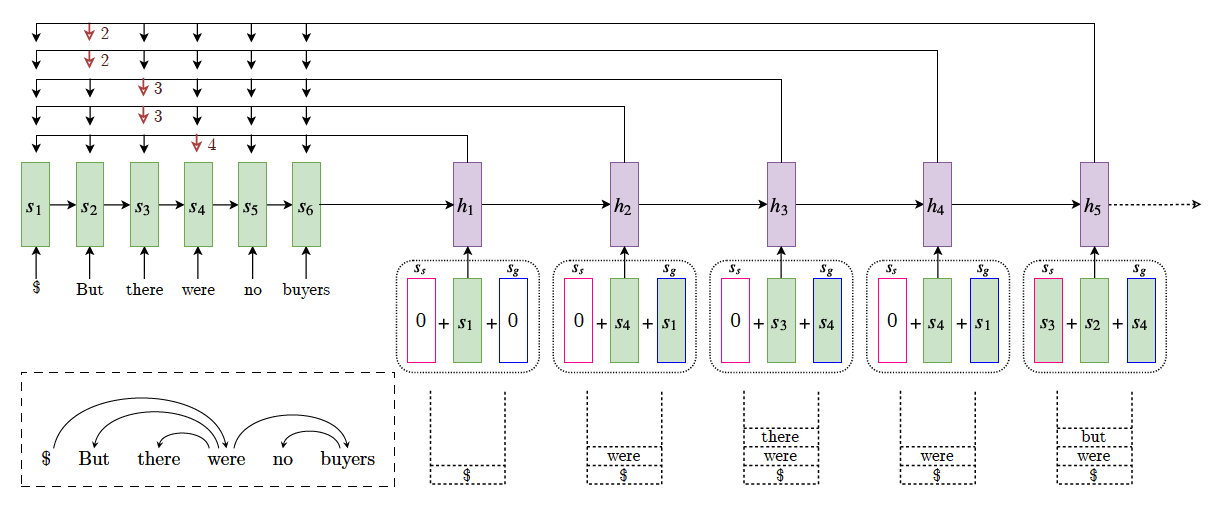
\includegraphics[scale=0.3]{img/chapter_nlp/parser_nn.png}
\label{fig:parser_nn}
\end{figure}


\subsection{应用案例}
依存语法分析在信息检索,评价抽取和情感分析等NLP任务上都有很多应用。比如“谢霆锋的儿子是谁”和
“谢霆锋是谁的儿子” 两句话如果不使用依存语法分析,很有可能就返回了一样的结果。依存句法分析能够更直接地通过语法结构的规则约束筛选出可能正确结果,提升相应任务的准确性。又比如“深圳大学非常漂亮,学生都很聪明”,这里 “漂亮” 形容的是 “深圳大学”, “聪明”形容的是“学生”,通过依存句法分析,就可以抽取出对应的搭配。再比如“我家音响声音很大”和“我家洗衣机声音很大”,两者在情感上前者是正评价,后者是负评价,需要使用依存句法分析来识别“声音很大”的修饰对象。

常用的中文依存句法分析的工具有复旦大学fnlp\footnote{\url{https://github.com/FudanNLP/fnlp}},斯坦福大学 Stanford CoreNLP\footnote{\url{https://stanfordnlp.github.io/CoreNLP/}}, Hanlp\footnote{\url{https://github.com/hankcs/HanLP}}和哈工大 LTP\footnote{\url{https://github.com/HIT-SCIR/ltp}}。





\section{语义分析}
在自然语言处理领域,语义分析涉及在某种程度上理解单词、短语、句子或文档的意义。传统狭义语义分析主要包括语义消歧(word sense disambiguation)\cite{ yarowsky1995unsupervised}和语义角色标注(semantic role labeling)\cite{ carreras2005introduction, bjorkelund2009multilingual}。语义消歧指在给定文本上下文中确定多义词语的含义,例如,“他买了一台新苹果,用来修图更方便了”中,苹果一次指代苹果电脑,而非水果。语义角色标注是给词语和短语标注其在上下文文本中的含义的过程,典型标注标签包括主体、意图、结果等。语义角色标注是面向任务型对话系统中核心组件自然语言解析模块的基础技术之一。
\begin{figure}[h]
\centering
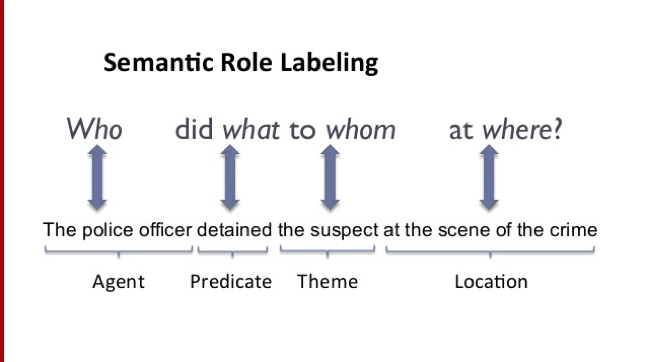
\includegraphics[scale=1]{img/chapter_nlp/guang_analysis_1.png}
\label{fig:universe}
\end{figure}
随着深度神经网络在自然语言处理领域的应用和研究,基于神经网络的语义分析得到了越来越多的应用和发展,并成为了驱动神经机器翻译\cite{ bahdanau2014neural, luong2015effective}、阅读理解\cite{ hermann2015teaching}、对话系统\cite{ serban2016building, chen2017survey}的最基础和核心的技术。基于神经网络的语义分析广义上可分为语义表示和语义匹配。其中语义表示任务将词语和短语镶嵌到高维向量空间中,称作词向量,作为CNN\cite{ lecun1995convolutional}、RNN\cite{ hochreiter1997long}和Transformer\cite{ vaswani2017attention}等模型的底层输入,根据任务需要,可以灵活的实现文本分类\cite{ joulin2016bag, zhang2015character}、机器翻译、阅读理解、对话系统、文本摘要\cite{ tan2017abstractive, yao2017recent}等自然语言处理任务,逐步替代或部分替代了传统以ngram one-hot向量作为底层表示的方法。语义匹配任务更多关注句子和篇章层级的语义的相似性,例如,寻找给定语料库中与查询语句语义层面最相似的句子。语义匹配任务在信息抽取、对话系统、问答系统都有广泛的应用。
\subsection{语义表示}
语义表示中词向量的概念可以追溯到Bengio的著作\cite{ bengio2003neural}。作者在文中提出了一种基于神经网络的语言模型,创新的提出将每一个词表示成一个高维的向量,而后使用神经网络计算给定上文词语后,下一个词出现的概率分布,最大化训练语聊出现的概率。训练语料是单词序列$w_1, \cdots, w_t, w_t \in V$,其中$V$是全体单词的集合。语言模型的目标是找到一个模型$f(w_t, \cdots, w_t-n+1) = P(w_t|w_1 ^ {t-1})$,即在给定前$t-1$个词的情况下,对第$t$个词的概率分布建模。Bengio提出把词表示成实数向量,$C(i) \in R^m$,即每一个词对应一个维度为$m$的实数向量,映射$C$可以用一个$|V| \times m$的实数矩阵表示。在第二步中,作者提出使用神经网络$g$来建模给定前缀序列下一个词的概率。
\begin{figure}[h!]
\centering
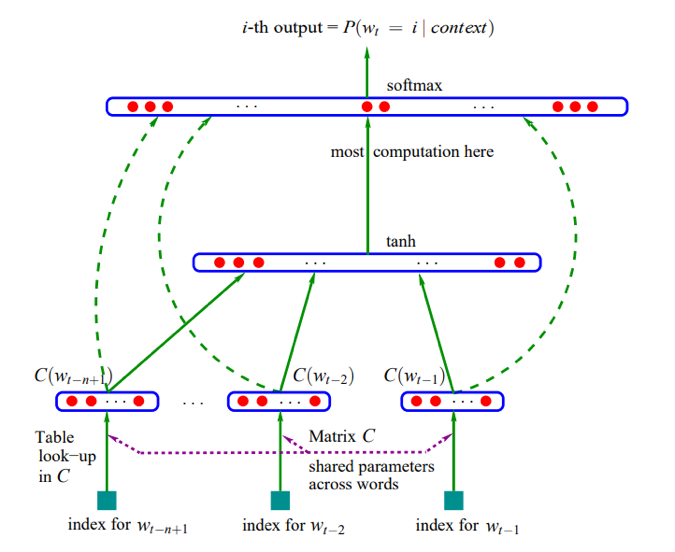
\includegraphics[scale=1]{img/chapter_nlp/guang_represent_1.png}
\label{fig:universe}
\end{figure}
其中,将词表示成高维实数向量的方法是词向量以及一系列神经网络在自然语言处理应用的开端。通常,我们会设计一个仅与文本结构或上下文相关的(无监督)任务作为目标,拟合训练数据,得到词向量表示。在Bengio之后,Word2Vec\cite{ mikolov2013distributed}, Glove\cite{ pennington2014glove}, ELMo\cite{ peters2018deep}等一系列词向量方法出现并逐渐成为自然语言处理的标准工具。
语义表示不仅限于词的层面,广义的语义表示在现代基于神经网络的自然语言处理中应用广泛。例如,神经机器翻译通常采用编码器译码器(Encoder-Decoder)\cite{ sutskever2014sequence}结构,其中编码器的输出可以看做是翻译模型对输入文本的语义表示,译码器基于该表示,生成目标语言的文本。再如,闲聊型对话系统中,需要针对聊天的上文给出合适的回答。闲聊对话系统可以分为生成式对话系统(Generation-based)\cite{ shang2015neural}和选择式对话系统(Selection-based)\cite{ chen2017survey}。选择式对话系统依赖语义匹配方法。典型的生成式闲聊对话系统也采用编码器译码器结构,其中编码器的输出是对聊天上文的总结性表示,可以认为是广义上的聊天上文的语义表示,用于在译码器中生成合适的回答语句。此外,随着自然语言处理预训练模型的发展,Bert\cite{devlin2018bert},GPT-2\cite{ radford2019language},MASS\cite{ song2019mass}等预训练模型(Pretrained models)在阅读理解等任务上大放异彩。这些模型可以看做是多个联合任务共享底层语义表示的学习,通常使用与文本结构相关的目标作为训练目标,设计神经网络结构表示文本。在应用时,这些预训练获得的表示仅需在少量标注数据上进行优化,即可获得优秀的子任务模型。通常,编码器和预训练模型采用CNN、RNN、Transformer等结构处理文本序列,在CNN和RNN中通常还会使用注意力(Attention)机制,得到文本片段的语义表示。

\subsection{语义匹配}
语义匹配任务在语义表示的基础上,对文本片段之间的相似度或相关度给出量化指标,语义越相似的片段匹配分数越高。语义匹配可大致分为基于表示的匹配(representation-based matching)\cite{ feng2015applying}和基于交互的匹配(interaction-based matching)\cite{ zhou2018multi, luspatio}。
基于表示的匹配方法注重对表示层的构建,将待匹配的对象通过语义表示的方法转换成等长的向量,并在此基础上进行匹配度计算。常见的匹配度计算方式包括cosine函数,和神经网络匹配。Cosine函数直接计算待匹配对的语义表示向量间的cosine值,通常cosine值越大代表待匹配对的相似度或相关度越高。这种方法不需要额外的训练数据,实现简单并且高效,在工业中广泛应用。神经网络匹配方式使用一个额外的神经网络结构,将待匹配对的语义表示向量作为输入,计算语义匹配分数。这种方法更加灵活,可根据数据定制匹配结构。但需要额外的标注数据进行训练,才能得到可用的匹配模型。
\begin{figure}[h!]
\centering
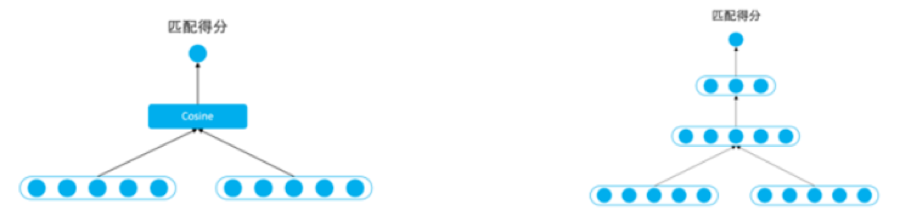
\includegraphics[scale=0.8]{img/chapter_nlp/guang_match_1.png}
\label{fig:universe}
\end{figure}
基于交互的匹配方法通常会保留待匹配对的序列信息,不会在表示层将文本转换成唯一的一个整体向量表示,而保留一个向量序列,用于接下来的交互匹配过程。例如将句子表示成一个与句子等长的向量序列。该向量序列可以使用语义表示的方法得到,例如使用RNN对文本序列进行建模。得到待匹配的序列对后,可以对序列中每个位置的向量计算与待匹配序列中向量的相关度。对每一个位置使用相同的方式计算相关度,可以得到一个匹配矩阵(matching matrix)。匹配矩阵包含了更细致的局部文本交互信息,在交互矩阵的寄出上,我们可以构建神经网络结构计算最终匹配得分,去拟合目标得分。下图\cite{ luspatio}展示了一个典型的基于交互的语义匹配方法在选择式对话系统中的结构。其中Representation module对应语义表示部分,matching block对应交互匹配部分。
\begin{figure}[h!]
\centering
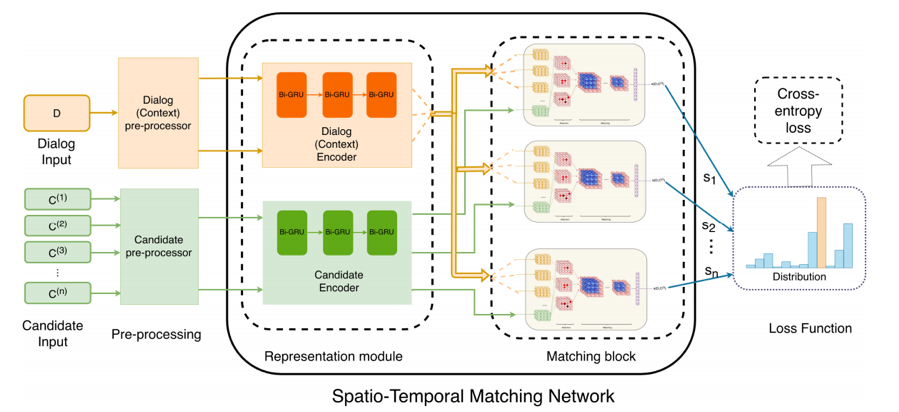
\includegraphics[scale=0.8]{img/chapter_nlp/guang_match_2.png}
\label{fig:universe}
\end{figure}

